% 03_markovnet.tex
In this section, we consider methods for exploiting temporal correlation between CSI of subsequent timeslots.
Assuming the channel does not change substantially within a certain window of time,
a reasonably accurate CSI estimate at some time $t-1$ can be used to estimate the CSI at time $t$.
Generically, we can write this estimator as
\begin{align}
\hat{\mathbf H}_t &= f(\hat{\mathbf H}_{t-1}) \label{eq:gen_estim}
\end{align}
Where $\mathbf{H}_i$ is the CSI matrix at time $t_i$ and $\hat{\mathbf H}_i$ is its estimator. 
This which admits an estimation error of 
\begin{align}
\mathbf E_{t} &= \mathbf H_{t} - \hat{\mathbf H}_{t}. \label{eq:diff_err}
\end{align}

\subsection{Related Work}

Non ML-based work in temporal correlation for CSI estimation utilized state-space methods such as the Kalman filter \cite{ref:Huber2006improved,ref:Ali2020BayesKalmanFilter,ref:Kim2021KalmanVsML}. Since it relies on explicit state space and noise models, the Kalman filter's predictive power in CSI estimation is limited. Furthermore, such work generally does not propose a method for feedback compression, making comparison with the following ML methods difficult.

Recent works have leveraged recurrent neural networks (RNNs) to exploit temporal correlation for CSI estimation \cite{ref:Lu2019RecCsiNet, ref:Liao2019BiLSTM, ref:Li2020SpatTempLSTM,
 ref:Jang2019Delay,ref:Wang2019CsiNetLSTM}. RNNs include recurrent layers, such as the long short-term memory (LSTM) cell or the gated recurrent unit (GRU), which are capable of learning long-term dependencies of a given process through backpropagation \cite{ref:Hermans2013Training} and can be used to predict future states of the process \cite{ref:Pascanu2014HowTo}.

\begin{figure}[htb]
	\centering
	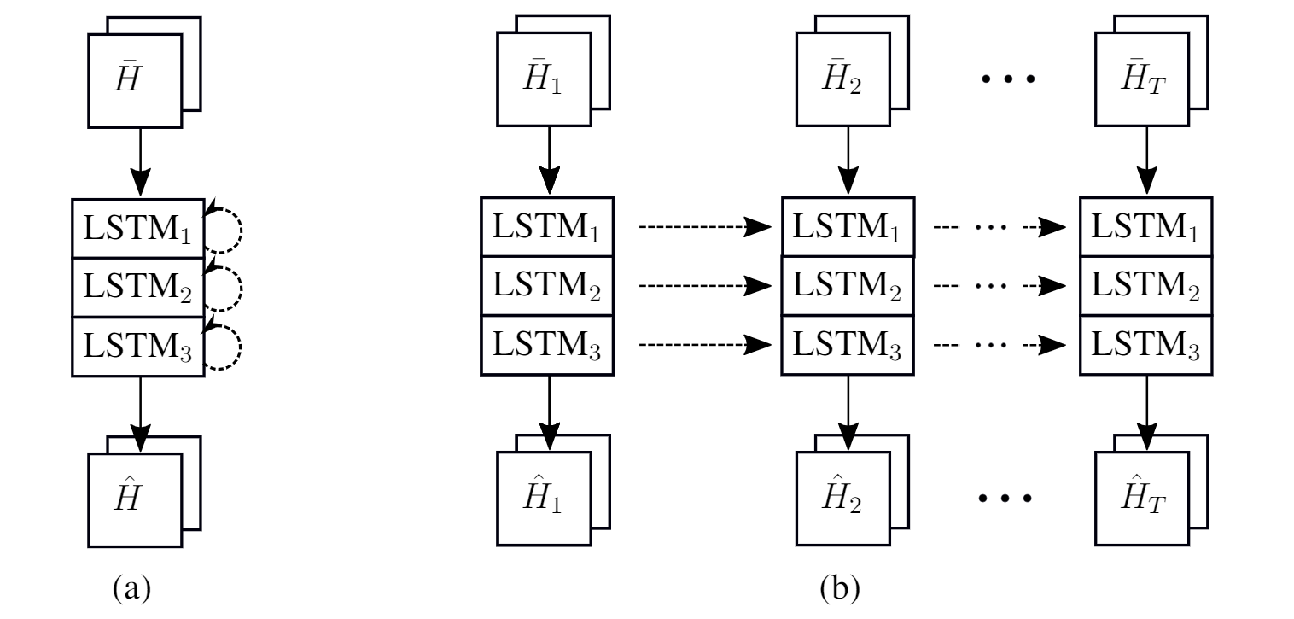
\includegraphics[width=.9\textwidth]{lstm-example-unroll.pdf}
	\medskip
	\caption{An example of LSTMs used for CSI estimation. (a) ``Stacked'' LSTM network of depth 3 shown with recurrent connections. (b) Same LSTM network ``unrolled" into $T$ timeslots }
	\label{fig:lstm_example}
\end{figure}

RNNs have been used extensively in natural language processing (NLP) for machine translation \cite{ref:Sutskever2014seq2seq} and sentiment extraction \cite{ref:Irsoy2014opinion}. For such works in NLP, authors have empirically found ``stacked'' or ``deep'' RNNs to be effective (e.g., Fig.~\ref{fig:lstm_example}), hypothesizing that having multiple recurrent layers allows the network to extract different semantic timescales \cite{ref:Irsoy2014opinion, ref:Bengio2009Learning}. Works in CSI estimation have taken cues from this work in NLP, proposing CSI estimation networks with stacked LSTMs after a sequence of autoencoders \cite{ref:Wang2019CsiNetLSTM}. While such work has demonstrated the utility of RNNs, the computational cost of LSTMs can be prohibitively high. For example, the RNN portion of the network proposed in \cite{ref:Wang2019CsiNetLSTM} accounts for $10^8$ additional parameters. Since channel estimation should not place an undue computational burden on the communications system, LSTMs can be problematic.

\subsection{Methods}

Rather than use RNNs to extract temporal dependencies in CSI data, we proposed a lightweight network based on the principle of differential encoding. We propose to train a network to estimate the error (\ref{eq:diff_err}) when using a simple linear estimator,
\begin{align*}
\hat{\mathbf H}_t &= \gamma \hat{\mathbf H}_{t-1} 
\end{align*}
where $\gamma$ is the minimum mean squared error (MMSE) estimator.
\begin{align*}
\mathbf H_t &= \gamma\mathbf H_{t-1} + \mathbf E_t \\
\mathbf H_{t-1}^H\mathbf H_t &= \gamma\mathbf H_{t-1}^H\mathbf H_{t-1} + \mathbf H_{t-1}^H\mathbf E_t \\
\end{align*}
Under the principle of orthogonality, the product $\mathbf H^H_{t-1}\mathbf E_t$ becomes a zero matrix. Denoting the cross correlation matrix as $\mathbf R_{i} = \mathbb{E}\left[\mathbf H_{t-i}^H\mathbf H_{t}\right]$.

\begin{align*}
\mathbf H_{t-1}^H\mathbf H_t &= \mathbf H_{t-1}^H\mathbf H_{t-1} 
\end{align*}

\subsubsection{Notation}

\subsubsection{Method Subsection \#1}
\label{sect:methods_sub1}

\subsubsection{Methods Subsection \#2}
\label{sect:methods_sub2}

